\RequirePackage{luatex85}
\documentclass[tikz,border=3.14mm]{standalone}
\usetikzlibrary{decorations.markings,arrows.meta,bending}

\begin{document}
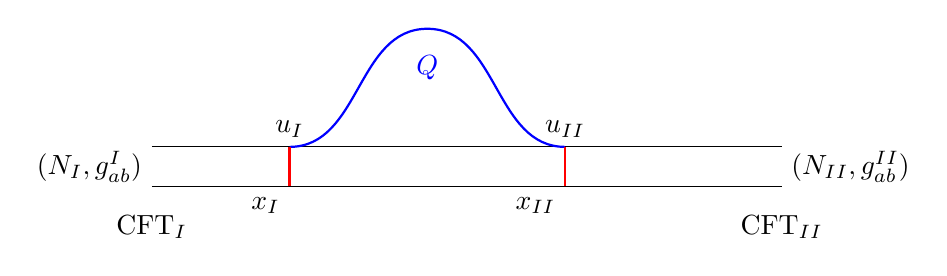
\begin{tikzpicture}[
    every label/.append style={font=\small},
     decoration={
        markings,% switch on markings
        mark=at position 0.5 with {\arrow{Straight Barb[bend]}}
    },
    postaction={decorate}
]

% draw the black lines
\draw (0,0) -- (8,0);
\draw (0,0.5) -- (8,0.5);

% labels
\node[below] at (0,-0.25) {CFT$_{\text{I}}$};
\node[below] at (8,-0.25) {CFT$_{\text{II}}$};

% the interface brane Q
\draw[blue,thick] (1.75,0.5) to[out=0,in=180] (3.5,2) to[out=0,in=180] (5.25,0.5);
\node[blue] at (3.5,1.5) {$Q$};

% vertical lines
\draw[red,thick] (1.75,0) -- (1.75,0.5);
\draw[red,thick] (5.25,0) -- (5.25,0.5);

% labels for the vertical lines
\node[left] at (1.75,-0.25) {$x_{\text{I}}$};
\node[left] at (5.25,-0.25) {$x_{\text{II}}$};

% labels for the vertical arrows
\node[above] at (1.75,0.5) {$u_{\text{I}}$};
\node[above] at (5.25,0.5) {$u_{\text{II}}$};

% labels for the left and right bulk
\node[left] at (0,0.25) {$(N_{\text{I}},g^{\text{I}}_{ab})$};
\node[right] at (8,0.25) {$(N_{\text{II}},g^{\text{II}}_{ab})$};

\end{tikzpicture}
\end{document}